\documentclass[12pt]{jarticle}
\usepackage{TUSIReport}
\usepackage{bm}
\usepackage{ascmac}
\usepackage{framed}
\usepackage[dvipdfmx]{graphicx}
\begin{document}
\提出者{情報工学実験2}{実験テーマ1 数理計画法}{2020}{9}{28}{4619060}{照永詩恩}
\共同実験者{}{}{}{}{}{}{}{}
\表紙出力
\section{実験の要旨}
最急降下法とニュートン法といった汎用性の高いアルゴリズムを実装し,理解を深めるとともに
非線形最適化問題への適応を通してアルゴリズムの特性を把握しておくことの重要性の理解を図る.
\section{実験の目的}
非線形最適化問題に対し,最急降下法を実装・適用を通し,アルゴリズムの特性を理解する.
\section{実験の原理(理論)}
\subsection{無制約最小化問題に対する基礎理論}
無制約最小化問題とは,$n$変数関数$f:\boldsymbol{R}^n \rightarrow \boldsymbol{R}$に対して定義される以下の問題である.
\begin{eqnarray}
    Minimize\ f(\boldsymbol(x))\ subject\ to\ \boldsymbol(x)=(x_1,x_2,\cdots,x_n)^T \in \boldsymbol{x}\nonumber
\end{eqnarray}
\subsubsection{諸定義}
$n$変数関数$f:\boldsymbol{R}^n \rightarrow \boldsymbol{R}$に対し勾配ベクトル$\nabla f(\boldsymbol{x}$とヘッセ行列$\nabla^2f(\boldsymbol{x})$はそれぞれ以下のように
定義されるベクトルと行列である.
\begin{eqnarray}
    \nabla f(\boldsymbol{x})=\left(\begin{array}{r}
        \frac{\partial f}{\partial x_1}\\
         \vdots \\
        \frac{\partial f}{\partial x_1}
    \end{array}\right),
    \nabla f^2(\boldsymbol{x})=\left(\begin{array}{rrr}
        \frac{\partial^2f}{\partial^2x_1}&\cdots&\frac{\partial^2f}{\partial x_1\partial x_n}\\
         \vdots &\ddots & \vdots \\
        \frac{\partial^2f}{\partial x_n\partial x_1}&\cdots&\frac{\partial^2f}{\partial^2x_n}   
    \end{array}\right)\nonumber
\end{eqnarray}
勾配ベクトルとヘッセ行列はそれぞれ1変数関数$f(\boldsymbol{x})$の微分係数$f'(\boldsymbol{x})$と2階微分係数$f''(\boldsymbol{x})$を
n変数関数に拡張したものである.ヘッセ行列は対称行列になることを注意する.勾配ベクトルとヘッセ行列は$f$のテイラー展開に現れる.具体的には,$x=a$の周りで2次の項まで求めると,以下のようになる.
\begin{eqnarray}
    f(\boldsymbol{a}+\boldsymbol{b})=f{\boldsymbol{a}}+\nabla f(\boldsymbol{a})^T\boldsymbol{d}+\frac{1}{2}\boldsymbol{d}^T\nabla^2f(\boldsymbol{a})\boldsymbol{d}+(残差)\nonumber
\end{eqnarray}
また,n次実正方行列$X$に対し,
\begin{itemize}
    \item $X$が半正定値とは,$X^T=X$と,$\forall\boldsymbol{d}\in\boldsymbol{R}^n$,$\boldsymbol{d}^TX\boldsymbol{d}\geq 0$が成り立つことを言い,
    \item $X$が半正定値とは,$X^T=X$と,$\forall\boldsymbol{d}\in\boldsymbol{R}^n\backslash \ \{\boldsymbol{0}\}$,$\boldsymbol{d}^TX\boldsymbol{d}> 0$が成り立つことを言う.
\end{itemize}
さらに,n次実行列$X$に対し,「$X$が半正定値$\Leftrightarrow$ $X$の固有値がすべて正」が成り立つ.
\subsubsection{最適性条件}
一般に非線形最適問題において大域的最適解を求めることは難しく,多くの場合は同署的最適解を求めることを目指す.局所最適解においては以下の最適性条件が成り立つ.
\begin{description}
    \item[定理(最適性の必要条件)] $\boldsymbol{x}^*\in \boldsymbol{R}^n$を無制約最小問題の極小的最適解として次が成り立つ.
    \begin{itemize}
        \item $f$が連続的微分可能$\Rightarrow \nabla f(\boldsymbol{x})^*=0$.
        \item $f$が2回連続微分可能$\Rightarrow \nabla f(\boldsymbol{x})^*$は半正定値行列.
    \end{itemize}
    1次の必要条件を満たす$\boldsymbol{x}^*$を停留点という.
    \item[定理(2次の十分条件)] 関数$f$が2回連続的微分可能とする.$\boldsymbol{x}^*\in \boldsymbol{R}^n$が以下の条件を満たすならば,$\boldsymbol{x}^*\in \boldsymbol{R}^n$
    は無制約最小化問題の極小的最適解である.
    \begin{itemize}
        \item $\nabla f(\boldsymbol{x}^*)=0$
        \item $\nabla^2f(\boldsymbol{x}^*)$が正定値行列
    \end{itemize}
    関数が凸性と呼ばれる「良い」性質を持つ場合には,実は,大域的最適解を求めることが比較的に容易になる.関数$f:\boldsymbol{R}^n\rightarrow \boldsymbol{R}$が異常の条件を満たすときは
    $f$が凸関数である.
    \begin{eqnarray}
        f(\lambda\boldsymbol{x}+(1-\lambda)\boldsymbol{y})\leq \lambda f(\boldsymbol{x})+(1-\lambda)f(\boldsymbol{y})\ \ \forall \boldsymbol{x},\boldsymbol{y}\in \boldsymbol{R}^n,\forall \lambda\in(0,1)\nonumber
    \end{eqnarray}
    $f$が2回連続的微分可能であるとき,以下の事実が成り立つ.
    \begin{center}
        $f$が凸関数 \ \ $\Leftrightarrow\ \ \nabla^2f(\boldsymbol{x})$が半正定値行列\ \ $\forall \boldsymbol{x}\in \boldsymbol{R}^n$ 
    \end{center}
    さらに,凸関数は次の「局所最適性=大域的最適性」を満たす.
    \begin{center}
        $f$が凸関数の時,$\boldsymbol{x}$が$f$の局所的最適解$\rightarrow$ $\boldsymbol{x}^*$は$f$の大域的最適解
    \end{center}
    これにより,微分可能な凸関数に対しては,$\nabla f(\boldsymbol{x})=0$を満たす$\boldsymbol{x}$を求めれば,その$\boldsymbol{x}^*$は
    最適解であることが保証される.凸関数はこのように重要なクラスである.
\end{description}
\subsubsection{反復法}
適当な初期点$x_0\in \boldsymbol{R}^n$からスタートし,以下の更新式で次々と点$x_1,x_2,\cdots,$を生成するアルゴリズムを反復法という.
\begin{eqnarray}
    x_{k+1}=x_k+\alpha_kd_k\nonumber
\end{eqnarray}
この式における$d_k$を探索方向,$\alpha_k$をステップ幅という.\\
\par 探索方向としては降下方向になっているものを用いるのが一般的である.$\nabla f(\boldsymbol{x})\neq 0$であれば,$-\nabla f(\boldsymbol{x})$
は自明な降下方向である.これを最急降下方向という.
\subsubsection{最急降下法}
最急降下法とは,$x_k$における最急降下方向を常に用いる方法である.手順は以下の通り.
\begin{enumerate}
    \item 初期点を選び,$k=0$とする.$\epsilon=10^{-8}$とする.
    \item $||\nabla f(\boldsymbol{x_k})||<\epsilon$が満たされていれば終了する.
    \item 探索方向を$d_k=-\nabla f(\boldsymbol{x_k})$とする.
    \item アルミホ条件による直線探索を用いてステップ幅$\alpha$を定める.
    \item $x_{k+1}=x_k+\alpha_kd_k$,$k=k+1$として(2)に戻る.
\end{enumerate}
\begin{description}
    \item[最急降下法の大域的収束性] 関数$f(\boldsymbol{x})$に関する仮定の下ではウルフ条件を用いた最急降下法は任意の初期店に対して以下の式が成り立つ. 
    \begin{eqnarray}
        \lim_{k\rightarrow \infty}||\nabla f(\boldsymbol{x}_k)||=0\nonumber
    \end{eqnarray}
    このように,初期店に依存せずに停留点に収束するのは最急降下法の強みであるがその一方で収束スピードが非常に遅い欠点を持つ. 
    \item[最急降下法の1次収束性] 最急降下法で生成される点列$\{\boldsymbol{x}_k\}$の収束先を$\boldsymbol{x}^*$とすると
    以下の式が成り立つ$0<c<1$が存在する.
    \begin{eqnarray}
        ||\boldsymbol{x}_{k+1}-\boldsymbol{x}^*||\leq c||\boldsymbol{x}_{k}-\boldsymbol{x}^*||\nonumber
    \end{eqnarray}
    この式では一見,収束が遅いように見えないが$||\boldsymbol{x}_{k+1}-\boldsymbol{x}^*$が非常に微小なため急降下法が収束するまでに要する反復数は非常に多い.
\end{description}
\subsubsection{ニュートン法}
ニュートン法は$f(\boldsymbol{x})$2次の項までのテイラー展開を最小化することを繰り返す方法である.以下のニュートン方程式を解くことで得られる.
\begin{eqnarray}
    \nabla^2f(\boldsymbol{x}_k)d=-\nabla f(\boldsymbol{x}_k)\nonumber
\end{eqnarray}
手順は以下の通り.
\begin{enumerate}
    \item 初期点を選び,$k=0$とする.$\epsilon=10^{-8}$とする.
    \item $||\nabla f(\boldsymbol{x_k})||<\epsilon$が満たされていれば終了する.
    \item ニュートン方程式を解いて$d_k$を求める.
    \item $x_{k+1}=x_k+\alpha_kd_k$,$k=k+1$として(2)に戻る.
\end{enumerate}
\begin{description}
    \item[ニュートン法の局所的2次収束性] 初期点を$\boldsymbol{x}^*$の十分近くに点を取ると,ニュートン法で生成される点列$\{x_k\}$は収束し,
    その収束先を$\boldsymbol{x}^*$とすると以下を満たす定数$c\geq 0$が存在する.  
    \begin{eqnarray}
        ||\boldsymbol{x}_{k+1}-\boldsymbol{x}^*||\leq c||\boldsymbol{x}_{k}-\boldsymbol{x}^*||^2\nonumber
    \end{eqnarray}
    1次収束と異なり,上の2次収束は非常に速い.一方で,初期店のとり方が悪ければニュートン法は収束しなかったり,局所最適解でない点に収束することもしばしばある.
\end{description}
\section{実験課題}
\begin{enumerate}
    \item 実験目的とアルゴリズムに関する数学的理論について概要を述べよ.
    \item 以下の2種類の2変数に対して最急降下法を実行するプログラムを完成させよ.
    \begin{eqnarray}
        f_1(x_1,x_2)&=&\frac{1}{2}
        \left(\begin{array}{r}
            x_1\\
            x_2
        \end{array}\right)^T\left(\begin{array}{rr}
            p&q\\
            q&r
        \end{array}\right)\left(\begin{array}{r}
            x_1\\
            x_2
        \end{array}\right)+\left(\begin{array}{r}
            c_1\\
            c_2
        \end{array}\right)^T\left(\begin{array}{r}
            x_1\\
            x_2
        \end{array}\right)+e^{(x_1-x_2)^2}\nonumber\\
        f_2(x_1,x_2)&=&\sum^4_{i=0}\sum^2_{j=0}a_{ij}x^i_1x^j_2\nonumber
    \end{eqnarray}
    \item プログラムを動かしてふるまいを観察して考察せよ.
    \item 上の関数に対してニュートン法のプログラムを完成せよ
    \item プログラムを動かしてふるまいを考察せよ.
\end{enumerate}
\section{結果}
\begin{enumerate}
    \item 上記より目的と理論は述べた.
    \item 付録にてソースコードを載せる.
    \item 各コード3つあるが1つ取り上げて表にする.\\
    \item ソースコードは付録にのせる
    \item それぞれのソースコードの結果を表にする.データが3つあるが一つを例に記載する.
\end{enumerate}
\begin{table}[h]
    \caption{kadai1.c}
    \begin{center}
        \begin{tabular}{|c|c|}
            \hline
            回数&23\\
            \hline
            位置&(0.827955,0.232528)\\
            \hline
            目的関数&-2.559041\\
            \hline
            勾配ベクトル&(0.000000,0.000000)\\
            \hline
            ノルム&0.000000\\
            \hline
        \end{tabular}
        \caption{kadai1\_2.cの結果(data60.txt)}
        \begin{tabular}{|c|c|}
            \hline
            回数&1000\\
            \hline
            位置&(-15.351735,-287.442815)\\
            \hline
            目的関数&-51647.764894\\
            \hline
            勾配ベクトル&(27.717200,10.962134)\\
            \hline
            ノルム&29.806234\\
            \hline
        \end{tabular}
        \caption{kadai2.cの結果(rand\_exp1.txt)}
        \begin{tabular}{|c|c|}
        \hline
        回数&16\\
        \hline
        位置&(0.827955,0.232528)\\
        \hline
        目的関数&-2.559041\\
        \hline
        勾配ベクトル&(0.000000,-0.000000)\\
        \hline
        ノルム&0.000000\\
        \hline
    \end{tabular}
    \caption{kadai2\_2.cの結果(rand\_quart2.txt)}
        \begin{tabular}{|c|c|}
            \hline
            回数&7\\
            \hline
            位置&(-14.729993,-248.869871)\\
            \hline
            目的関数&-31254.330351\\
            \hline
            勾配ベクトル&(0.000000,0.000000)\\
            \hline
            ノルム&0.000000\\
            \hline
        \end{tabular}
    \end{center}
\end{table}
\section{検討・考察}
\subsubsection{最急降下法のプログラムの実行結果について}
それぞれ最急降下法のソースコードの目的関数の動きをグラフにした.
\begin{center}
    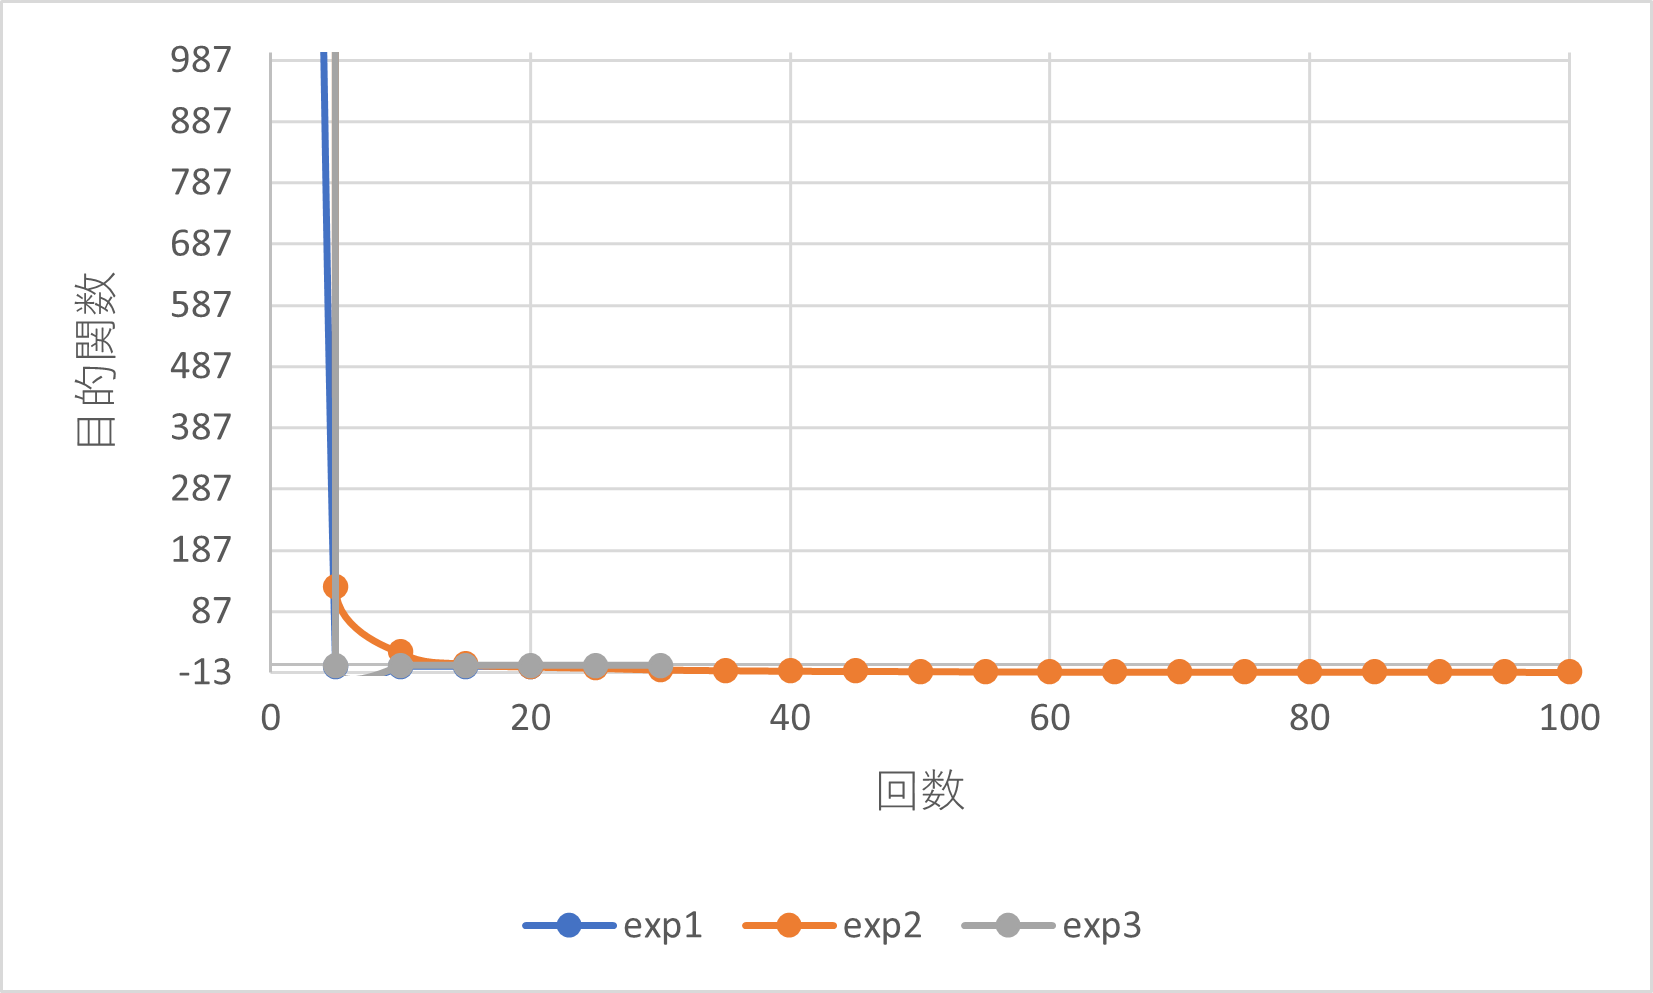
\includegraphics[width=15cm,clip]{1.png}\\
    図1.kadai1.cにおいてそれぞれのデータの目的関数の動き\\
\end{center}
\begin{center}
    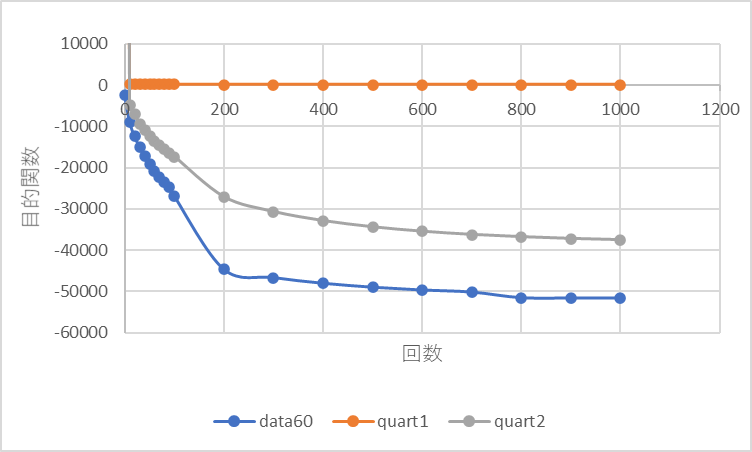
\includegraphics[width=15cm,clip]{2.png}\\
    図2.kadai1\_1.cにおいてそれぞれのデータの目的関数の動き\\
\end{center}
各図よりそれぞれとある値に収束すると考察した.\\
\subsubsection{ニュートン法のプログラムの実行結果について}
それぞれのニュートン法のソースコードの目的関数の動きをグラフにした.\\
\begin{center}
    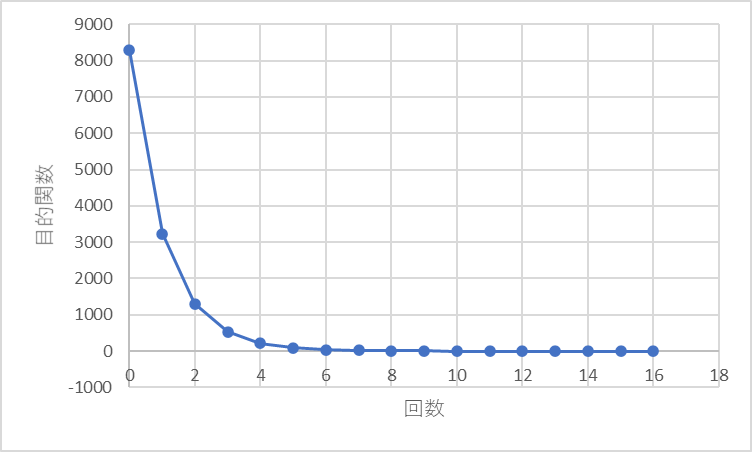
\includegraphics[width=15cm,clip]{3.png}\\
    図3.kadai2.cにおいてそれぞれのデータの目的関数の動き\\
\end{center}
\begin{center}
    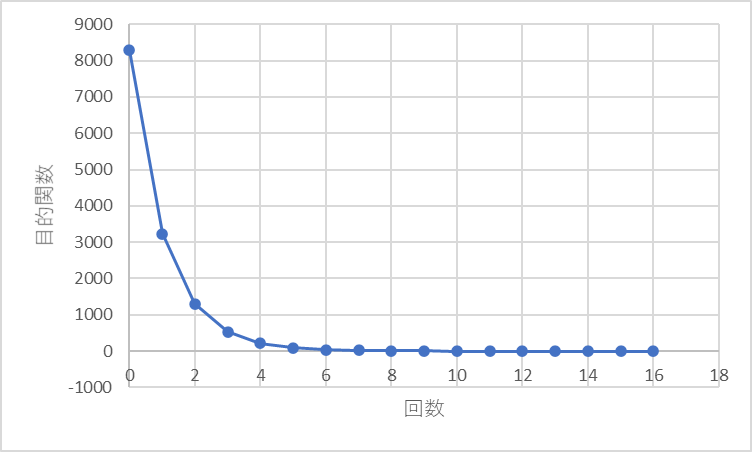
\includegraphics[width=15cm,clip]{3.png}\\
    図4.kadai2\_2.cにおいてそれぞれのデータの目的関数の動き\\
\end{center}
各グラフより目的関数はとある値に収束している.また,データの値によって
ヘッセ行列が正則でない場合が出てきてしまうこともあることもあると考える.
また,最急降下法と比較してみるとニュートン法の方が収束するときの回数が早いが,
ヘッセ行列が正則でないと正しい値が出ないためその点に関しては最急降下法に劣っている
と考えた.
\subsubsection{凸かどうかについて}
\begin{center}
    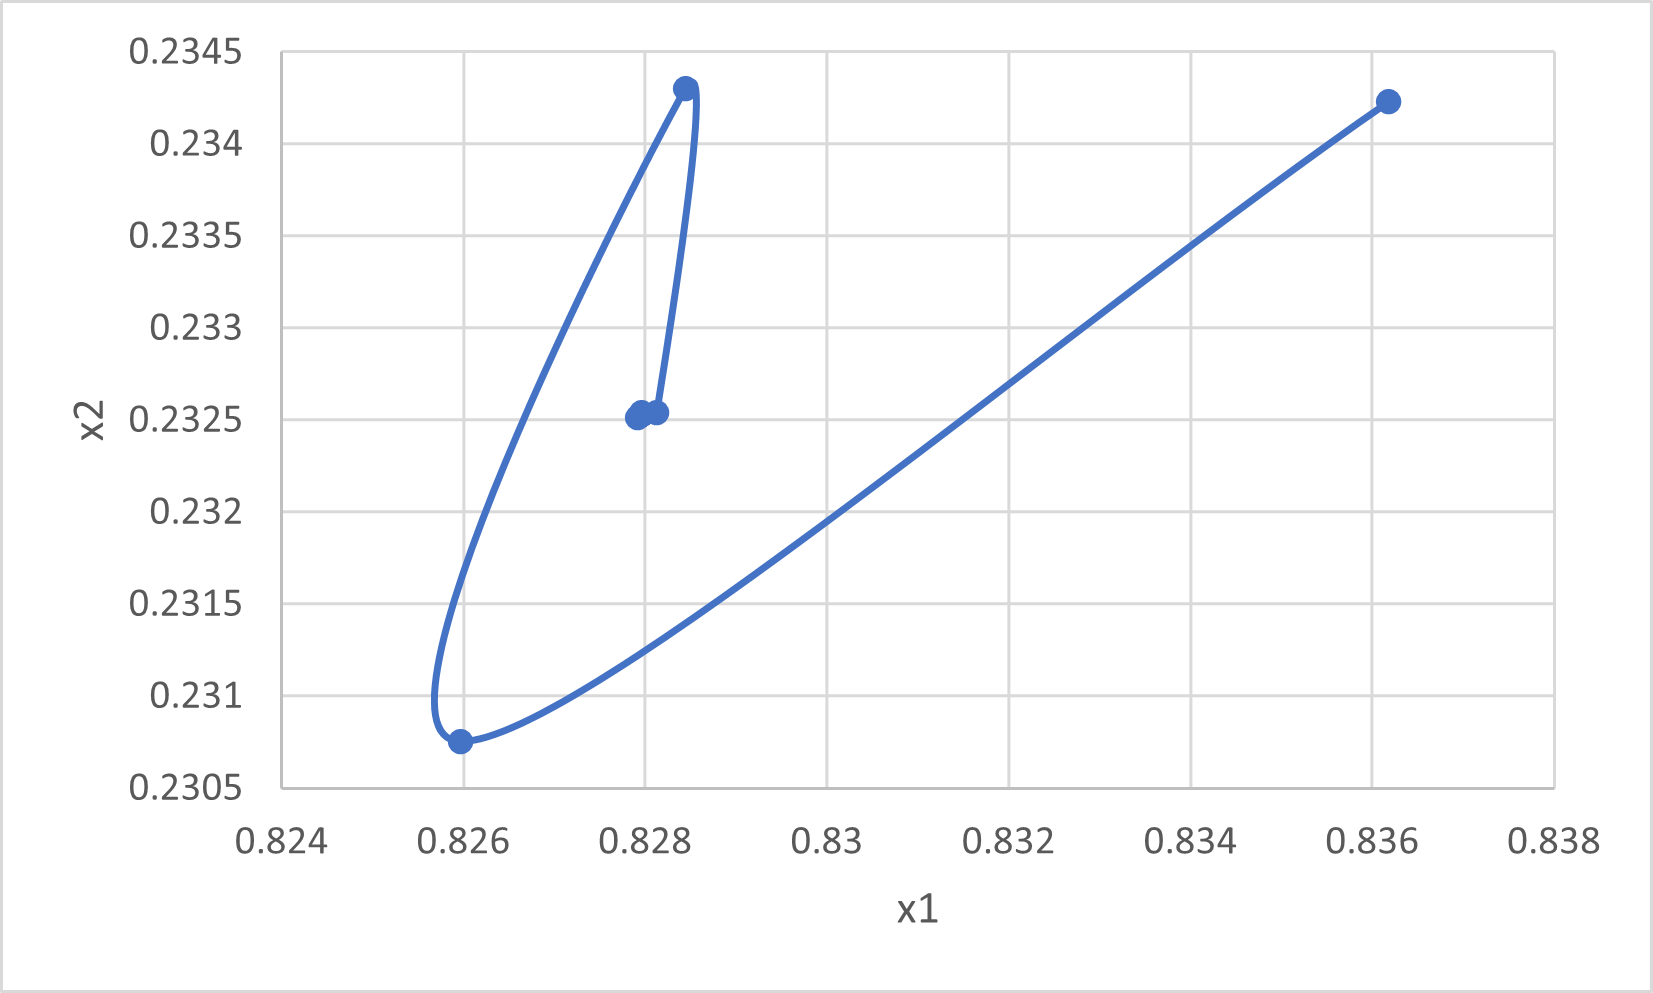
\includegraphics[width=15cm,clip]{5.png}\\
    図5.最急降下法の($x_1-x_2$)平面,rand\_exp1.txtより\\
\end{center}
\begin{center}
    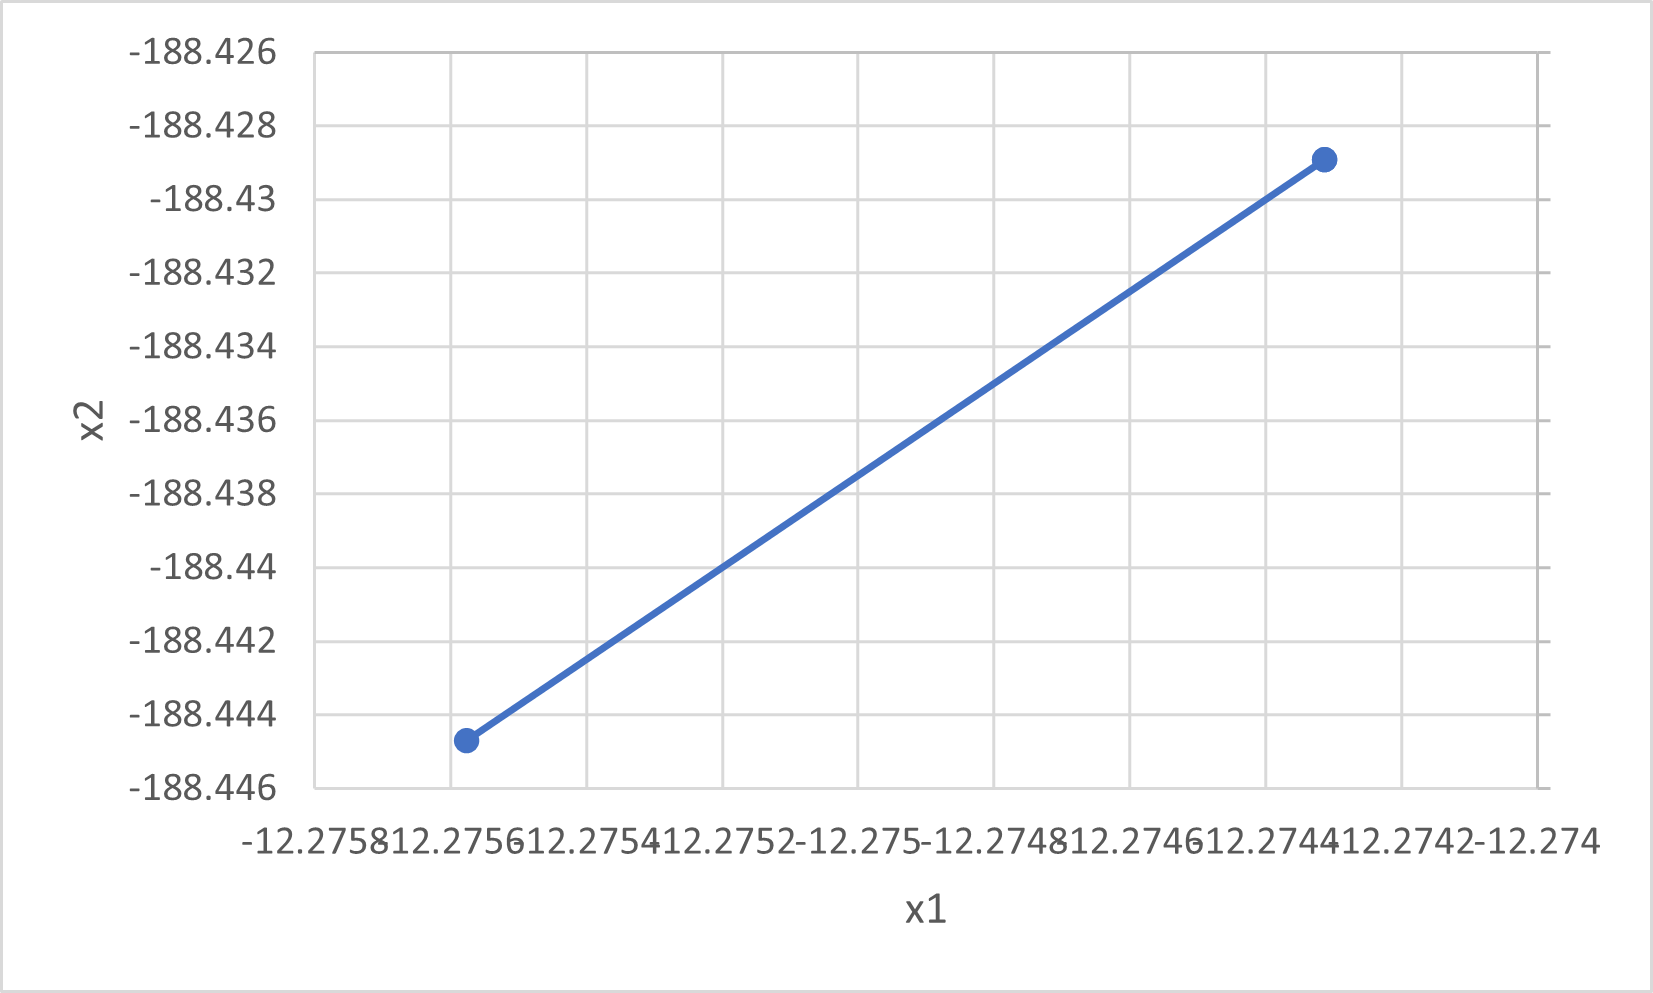
\includegraphics[width=15cm,clip]{6.png}\\
    図6.ニュートン法の($x_1-x_2$)平面,rand\_quart1.txtより\\
\end{center}
それぞれ,$f_1$,$f_2$関数のデータを1つずつ実行してノルムが大幅に小さくなった時に
現在の位置をプロットした.図5より最急降下法の法で使ったデータにおいては放物線のような
形となったため凸性ではないかと考察した.逆にニュートン法に用いたデータは直線のようになったため
これは凸性ではないと考えた.
\section{結論}
最急降下法とニュートン法のプログラムを実際に書いて適応することができ
さらにその仕組みを知ることができた.またこれらのことを通してアルゴリズムの特性を学ぶことができた.
% 参考文献
\begin{thebibliography}{99}
\label{sannkoubunnkenn_chapter}
\bibitem{rikadai}
情報工学実験2,
東京理科大学 工学部 情報工学科, 2020.
\end{thebibliography}
\clearpage
% 付録
\appendix
\section{付録}
\begin{framed}
    \begin{verbatim}
#include<stdio.h>
#include<stdlib.h>
#include<string.h>
#include<math.h>//expとpowを使うため
#define N 1000//反復回数の最大
#define eps 0.00000001
double M[2][2];
double C[2];
double function(double *x);//目的関数
double Armijo(double *x,double *d,double *g);//アルミホ条件
int main()
{
    int i,j,k;
    double alpha;
    char fname[128];
    double x[2];
    double p,q,r;
    double g[3],d[2],norm; 
    double f;             
    FILE *fp;                     
    //データのファイル操作
    printf("input filename:");
    fgets(fname,sizeof(fname),stdin);
    fname[strlen(fname)-1] = '\0';
    fflush(stdin);
    fp = fopen(fname, "r");
    for(i=0;i<2;i++)
    {
        for(j=0;j<2;j++)
        {
            fscanf(fp, "%lf", &M[i][j]); 
        } 
    }
    for(i=0;i<2;i++)
    {
        fscanf(fp, "%lf", &C[i]); 
    }
    for(i=0;i<2;i++)
    {
        
        fscanf(fp, "%lf", &x[i]); 
    }
    fclose(fp);
    //初期化表示
    printf("Q=\n");
    for(i=0;i<2;i++)
    {
        for(j=0;j<2;j++)
        {
            printf("%5.lf",M[i][j]);
        }
        printf("\n");
    }
    printf("C=\n");
    for(i=0;i<2;i++)
    {
        printf("%5.lf",C[i]);
    }
    printf("\n");
    printf("x=\n");
    for(i=0;i<2;i++)
    {
        printf("%5.lf",x[i]);
    }
    printf("\n");
    printf("------------------------------------\n");
    //ここから開始
    k=0;
    p=M[0][0];
    q=M[0][1];
    r=M[1][1];
    while(1)
    {
        //勾配ベクトル
        g[0]=p*x[0]+q*x[1]+C[0]+2*(x[0]-x[1])*exp(pow(x[0]-x[1],2));
        g[1]=r*x[1]+q*x[0]+C[1]-2*(x[0]-x[1])*exp(pow(x[0]-x[1],2));
        //探索方向
        d[0]=-g[0];
        d[1]=-g[1];
        norm=sqrt((pow(g[0],2)+pow(g[1],2)));
        f=function(x);
        alpha=Armijo(x,d,g);
        if(norm<eps)
        {
            break;
        }
        if(k<=100&&k%5==0)
        {
            printf("%d回目\n",k);
            printf("現在の位置=(%lf,%lf)\n目的関数=%lf\n勾配ベクトル=(%lf,%lf)\n,
            ノルム=%lf\n",x[0],x[1],f,g[0],g[1],norm);
            printf("------------------------------------\n");
        }
        else if(k>100&&k%100==0)
        {
            printf("%d回目\n",k);
            printf("現在の位置=(%lf,%lf)\n目的関数=%lf\n勾配ベクトル=(%lf,%lf)\n,
            ノルム=%lf\n",x[0],x[1],f,g[0],g[1],norm);
            printf("------------------------------------\n");
        }
        
        x[0]=x[0]+alpha*d[0];
        x[1]=x[1]+alpha*d[1];
        k++;
        if(k>N)
        {
            break;
        }
    }
    printf("最終結果\n");
    printf("回数=%d\n現在の位置=(%lf,%lf)\n目的関数=%lf\n
    勾配ベクトル=(%lf,%lf)\n,ノルム=%lf\n",
    k-1,x[0],x[1],f,g[0],g[1],norm);
    return 0;
}
double function(double *x)
{
    double fun;
    double p,q,r;
    p=M[0][0];
    q=M[0][1];
    r=M[1][1];
    fun=0.5*(p*pow(x[0],2)+2*q*x[0]*x[1]
    +r*pow(x[1],2))+C[0]*x[0]+C[1]*x[1]+exp(pow((x[0]-x[1]),2));
    return fun;
}
double Armijo(double *x,double *d,double *g)
{
    double alpha=1.0;
    double xi=0.1;
    double tau=0.5;
    double f1,f2,f3;
    double z;
    double p,q,r;
    double y[2];
    p=M[0][0];
    q=M[0][1];
    r=M[1][1];    
    while(1)
    {
        y[0]=x[0]+alpha*d[0];
        y[1]=x[1]+alpha*d[1];
        f1=function(y);
        f2=function(x);
        z=xi*(g[0]*d[0]+g[1]*d[1])*alpha;
        if(f1<=f2+z)
        {
            break;
        }
        else
        {
            alpha=tau*alpha;
        }
    }
    return alpha;
} 
    \end{verbatim}
\end{framed}
\begin{center}
    図A.1:最急降下法$f_1$のソースコード
\end{center}
\begin{framed}
    \begin{verbatim}
#include<stdio.h>
#include<stdlib.h>
#include<string.h>
#include<math.h>
#define N 1000
#define eps 0.00000001
double M[5][3];
double function(double *x);
double Armijo(double *x,double *d,double *g);
int main()
{
    int i,j,k;
    double alpha;
    char fname[128];
    double x[2];
    double p,q,r;
    double g[3],d[2],norm; 
    double f;             
    FILE *fp;                     

    printf("input filename:");
    fgets(fname,sizeof(fname),stdin);
    fname[strlen(fname)-1] = '\0';
    fflush(stdin);
    fp = fopen(fname, "r");
    for(i=0;i<5;i++)
    {
        for(j=0;j<3;j++)
        {
            fscanf(fp, "%lf", &M[i][j]); 
        } 
    }
    for(i=0;i<2;i++)
    {
        fscanf(fp, "%lf", &x[i]); 
    }
    fclose(fp);
    //初期化表示
    printf("a=\n");
    for(i=0;i<5;i++)
    {
        for(j=0;j<3;j++)
        {
            printf("%5.lf",M[i][j]);
        }
        printf("\n");
    }
    printf("x=\n");
    for(i=0;i<2;i++)
    {
        printf("%5.lf",x[i]);
    }
    printf("\n");
    printf("------------------------------------\n");
    k=0;
    while(1)
    {
        g[0]=M[1][0]+M[1][1]*x[1]+2*M[2][0]*x[0]+3*M[3][0]
        *pow(x[0],2)+4*M[4][0]*pow(x[0],3);
        g[1]=M[0][1]+2*M[0][2]*x[1]+M[1][1]*x[0];
        norm=sqrt((pow(g[0],2)+pow(g[1],2)));
        f=function(x);
        d[0]=-g[0];
        d[1]=-g[1];
        alpha=Armijo(x,d,g);
        if(norm<eps)
        {
            break;
        }
        if(k<=100&&k%10==0)
        {
            printf("%d回目\n",k);
            printf("現在の位置=(%lf,%lf)\n目的関数=%lf\n勾配ベクトル=(%lf,%lf)\n,
            ノルム=%lf\n",x[0],x[1],f,g[0],g[1],norm);
            printf("------------------------------------\n");
        }
        else if(k>100&&k%100==0)
        {
            printf("%d回目\n",k);
            printf("現在の位置=(%lf,%lf)\n目的関数=%lf\n勾配ベクトル=(%lf,%lf)\n,
            ノルム=%lf\n",x[0],x[1],f,g[0],g[1],norm);
            printf("------------------------------------\n");
        }
        
        x[0]=x[0]+alpha*d[0];
        x[1]=x[1]+alpha*d[1];
        k++;
        if(k>N)
        {
            break;
        }
    }
    printf("最終結果\n");
    printf("回数=%d\n現在の位置=(%lf,%lf)\n目的関数=%lf\n
    勾配ベクトル=(%lf,%lf)\n,ノルム=%lf\n",k-1,x[0],x[1],f,g[0],g[1],norm);
    return 0;
}
double function(double *x)
{
    double fun;
    fun=M[0][1]*x[1]+M[0][2]*pow(x[1],2)+M[1][0]*x[0]+M[1][1]*x[0]*x[1]
    +M[2][0]*pow(x[0],2)+M[3][0]*pow(x[0],3)+M[4][0]*pow(x[0],4);
    return fun;
}
double Armijo(double *x,double *d,double *g)
{
    double alpha=1.0;
    double xi=0.1;
    double tau=0.5;
    double f1,f2,f3;
    double z;
    double y[2];    
    while(1)
    {
        y[0]=x[0]+alpha*d[0];
        y[1]=x[1]+alpha*d[1];
        f1=function(y);
        f2=function(x);
        z=xi*(g[0]*d[0]+g[1]*d[1])*alpha;
        if(f1<=f2+z)
        {
            break;
        }
        else
        {
            alpha=tau*alpha;
        }
    }
    return alpha;
} 

    \end{verbatim}
\end{framed}
\begin{center}
    図A.2:最急降下法$f_2$のソースコード
\end{center}
\begin{framed}
    \begin{verbatim}
#include<stdio.h>
#include<stdlib.h>
#include<string.h>
#include<math.h>
#define inf 10000000000000
#define N 500
#define eps 0.00000001
double M[2][2];
double C[2];
double h[2][2];
double function(double *x);
double h_s(double *x,double *d);//ヘッセ行列を求める
double N_T(double *x,double *d,double *g);
int main()
{
    int i,j,k;
    char fname[128];
    double x[2];
    double p,q,r;
    double g[2],d[2],norm; 
    double f;             
    FILE *fp;                     
    //ファイル操作
    printf("input filename:");
    fgets(fname,sizeof(fname),stdin);
    fname[strlen(fname)-1] = '\0';
    fflush(stdin);
    fp = fopen(fname, "r");
    for(i=0;i<2;i++)
    {
        for(j=0;j<2;j++)
        {
            fscanf(fp, "%lf", &M[i][j]); 
        } 
    }
    for(i=0;i<2;i++)
    {
        fscanf(fp, "%lf", &C[i]); 
    }
    for(i=0;i<2;i++)
    {
        
        fscanf(fp, "%lf", &x[i]); 
    }
    fclose(fp);
    //初期化表示
    printf("Q=\n");
    for(i=0;i<2;i++)
    {
        for(j=0;j<2;j++)
        {
            printf("%5.lf",M[i][j]);
        }
        printf("\n");
    }
    printf("C=\n");
    for(i=0;i<2;i++)
    {
        printf("%5.lf",C[i]);
    }
    printf("\n");
    printf("x=\n");
    for(i=0;i<2;i++)
    {
        printf("%5.lf",x[i]);
    }
    printf("\n");
    printf("------------------------------------\n");
    //ここから開始
    k=0;
    p=M[0][0];
    q=M[0][1];
    r=M[1][1];
    while(1)
    {
        g[0]=p*x[0]+q*x[1]+C[0]+2*(x[0]-x[1])*exp(pow(x[0]-x[1],2));
        g[1]=r*x[1]+q*x[0]+C[1]-2*(x[0]-x[1])*exp(pow(x[0]-x[1],2));
        N_T(x,d,g);
        norm=sqrt((pow(g[0],2)+pow(g[1],2)));
        f=function(x);
        if(norm<eps||d[0]==inf)
        {
            break;
        }
        
            printf("%d回目\n",k);
            printf("現在の位置=(%lf,%lf)\n目的関数=%lf\n勾配ベクトル=(%lf,%lf)\n
            ,ノルム=%lf\n",x[0],x[1],f,g[0],g[1],norm);
            printf("------------------------------------\n");
        
        
        x[0]=x[0]+d[0];
        x[1]=x[1]+d[1];
        if(k>N)
        {
            break;
        }
        k++;
    }
    printf("最終結果\n");
    printf("回数=%d\n現在の位置=(%lf,%lf)\n目的関数=%lf\n勾配ベクトル=(%lf,%lf)\n,
    ノルム=%lf\n",k,x[0],x[1],f,g[0],g[1],norm);
    return 0;
}
double function(double *x)
{
    double fun;
    double p,q,r;
    p=M[0][0];
    q=M[0][1];
    r=M[1][1];
    fun=0.5*(p*pow(x[0],2)+2*q*x[0]*x[1]+r*pow(x[1],2))
    +C[0]*x[0]+C[1]*x[1]+exp(pow((x[0]-x[1]),2));
    return fun;
}
double h_g(double *x,double *d)
{
    double p,q,r;
    p=M[0][0];
    q=M[0][1];
    r=M[1][1];
    h[0][0]=p+2*exp(pow(x[0]-x[1],2))*(1+2*pow(x[0]-x[1],2));
    h[0][1]=q-2*exp(pow(x[0]-x[1],2))*(1+2*pow(x[0]-x[1],2));
    h[1][0]=h[0][1];
    h[1][1]=r+2*exp(pow(x[0]-x[1],2))*(1+2*pow(x[0]-x[1],2));
}
double N_T(double *x,double *d,double *g)
{
    double h_gg[2][2];
    h_g(x,d);
    if(h[0][0]*h[1][1]-h[0][1]*h[1][0]==0)//正則かどうかの判定
    {
        d[0]=inf;
        d[1]=inf;
        printf("非正則\n");
    }
    else
    {
        h_gg[0][0]=1/(h[0][0]*h[1][1]-h[0][1]*h[1][0])*h[1][1];
        h_gg[1][0]=1/(h[0][0]*h[1][1]-h[0][1]*h[1][0])*-h[1][0];
        h_gg[1][1]=1/(h[0][0]*h[1][1]-h[0][1]*h[1][0])*h[0][0];
        h_gg[0][1]=1/(h[0][0]*h[1][1]-h[0][1]*h[1][0])*-h[0][1];
        d[0]=-g[0]*h_gg[0][0]-g[1]*h_gg[1][0];
        d[1]=-g[0]*h_gg[0][1]-g[1]*h_gg[1][1];
    }
} 
    \end{verbatim}
\end{framed}
\begin{center}
    図A.3:ニュートン法$f_1$に関するソースコード
\end{center}
\begin{framed}
    \begin{verbatim}
#include<stdio.h>
#include<stdlib.h>
#include<string.h>
#include<math.h>
#define inf 10000000000000
#define N 500
#define eps 0.00000001
double M[5][3];
double h[2][2];
double function(double *x);
void h_s(double *x,double *d);
void N_T(double *x,double *d,double *g);
int main()
{
    int i,j,k;
    char fname[128];
    double x[2];
    double p,q,r;
    double g[2],d[2],norm; 
    double f;             
    FILE *fp;                     

    printf("input filename:");
    fgets(fname,sizeof(fname),stdin);
    fname[strlen(fname)-1] = '\0';
    fflush(stdin);
    fp = fopen(fname, "r");
    for(i=0;i<5;i++)
    {
        for(j=0;j<3;j++)
        {
            fscanf(fp, "%lf", &M[i][j]); 
        } 
    }
    for(i=0;i<2;i++)
    {
        
        fscanf(fp, "%lf", &x[i]); 
    }
    fclose(fp);
    //初期化表示
    printf("Q=\n");
    for(i=0;i<5;i++)
    {
        for(j=0;j<3;j++)
        {
            printf("%5.lf",M[i][j]);
        }
        printf("\n");
    }
    printf("x=\n");
    for(i=0;i<2;i++)
    {
        printf("%5.lf",x[i]);
    }
    printf("\n");
    printf("------------------------------------\n");
    k=0;
    p=M[0][0];
    q=M[0][1];
    r=M[1][1];
    while(1)
    {
        g[0]=M[1][0]+M[1][1]*x[1]+2*M[2][0]*x[0]+3*M[3][0]
        *pow(x[0],2)+4*M[4][0]*pow(x[0],3);
        g[1]=M[0][1]+2*M[0][2]*x[1]+M[1][1]*x[0];
        N_T(x,d,g);
        norm=sqrt((pow(g[0],2)+pow(g[1],2)));
        f=function(x);
        if(norm<eps||d[0]==inf)
        {
            break;
        }
            printf("%d回目\n",k);
            printf("現在の位置=(%lf,%lf)\n目的関数=%lf\n勾配ベクトル=(%lf,%lf)\n
            ,ノルム=%lf\n",x[0],x[1],f,g[0],g[1],norm);
            printf("------------------------------------\n");
        
        x[0]=x[0]+d[0];
        x[1]=x[1]+d[1];
        if(k>N)
        {
            break;
        }
        k++;
    }
    printf("最終結果\n");
    printf("回数=%d\n現在の位置=(%lf,%lf)\n目的関数=%lf\n
    勾配ベクトル=(%lf,%lf)\n,ノルム=%lf\n",k,x[0],x[1],f,g[0],g[1],norm);
    return 0;
}
double function(double *x)
{
    double fun;
    fun=M[0][1]*x[1]+M[0][2]*pow(x[1],2)+M[1][0]*x[0]+M[1][1]*
    x[0]*x[1]+M[2][0]*pow(x[0],2)+M[3][0]*pow(x[0],3)
    +M[4][0]*pow(x[0],4);
    return fun;
}
void h_g(double *x,double *d)
{
    double p,q,r;
    h[0][0]=2*M[2][0]+6*M[3][0]*x[0]+12*M[4][0]*pow(x[0],2);
    h[0][1]=M[1][1];
    h[1][0]=M[1][1];
    h[1][1]=2*M[0][2];
}
void N_T(double *x,double *d,double *g)
{
    double h_gg[2][2];
    h_g(x,d);
    if(h[0][0]*h[1][1]-h[0][1]*h[1][0]==0)
    {
        d[0]=inf;
        d[1]=inf;
        printf("非正則\n");
    }
    else
    {
        h_gg[0][0]=1/(h[0][0]*h[1][1]-h[0][1]*h[1][0])*h[1][1];
        h_gg[1][0]=1/(h[0][0]*h[1][1]-h[0][1]*h[1][0])*-h[1][0];
        h_gg[1][1]=1/(h[0][0]*h[1][1]-h[0][1]*h[1][0])*h[0][0];
        h_gg[0][1]=1/(h[0][0]*h[1][1]-h[0][1]*h[1][0])*-h[0][1];
        d[0]=-g[0]*h_gg[0][0]-g[1]*h_gg[1][0];
        d[1]=-g[0]*h_gg[0][1]-g[1]*h_gg[1][1];
    }
} 
    \end{verbatim}
\end{framed}
\begin{center}
    図A.4:ニュートン法$f_2$に関するソースコード
\end{center}
\end{document}